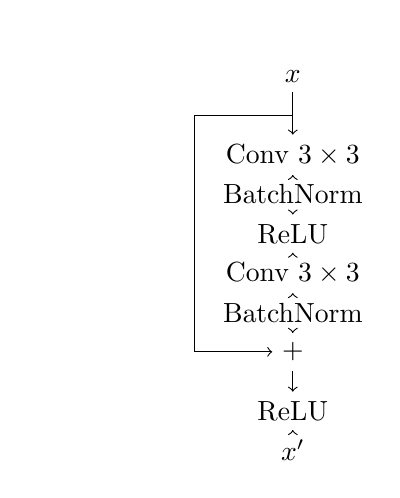
\begin{tikzpicture}[]
    % Nodes
    \node at (1.75,0) (input){$x$};
    \node[align=center] (conv1) at (1.75, -1) {\Th{Conv} $3\times3$};
    \node[align=center] (bn1) at (1.75, -1.5) {\Th{BatchNorm}};
    \node[align=center] (relu1) at (1.75, -2.0) {\Th{ReLU}};
    \node[align=center] (conv2) at (1.75, -2.5) {\Th{Conv} $3\times3$};
    \node[align=center] (bn2) at (1.75, -3) {\Th{BatchNorm}};
    \node[align=center] (sum) at (1.75, -3.5) {$+$};
    \node[align=center] (relu2) at (1.75, -4.25) {\Th{ReLU}};
    \node(output) at (1.75, -4.75) {$x'$};
    \node at (1.75,-0.5) (empt0) {};
    \node at (0.5, -2.5) (empt1) {};
    \node at (-1.5, 0.5) (emptkek) {};  

    %% CNN Edges
    \draw[->] (input.south) -- node {} (conv1);
    \draw[->] (conv1.south) -- node  {} (bn1.north);
    \draw[->] (bn1.south) -- node  {} (relu1.north);
    \draw[->] (relu1.south) -- node  {} (conv2.north);
    \draw[->] (conv2.south) -- node  {} (bn2.north);
    \draw[->] (bn2.south) -- node  {} (sum.north); 
    \draw[-] (empt0.center) -| node {} (empt1.center);
    \draw[->] (empt1.center) |- node {} (sum.west);
    \draw[->] (sum.south) -- node  {} (relu2.north);
    \draw[->] (relu2.south) -- node  {} (output.north);
\end{tikzpicture}
